\documentclass[table]{beamer}

\usepackage[spanish]{babel}
\usepackage[normalem]{ulem}
\usepackage{xcolor}
\usepackage{pgfgantt}
\usepackage{booktabs}
\usepackage{bookmark}
\usepackage{tabularx}
\usepackage{graphicx}
\usepackage{pgfplots}
\usepackage{multicol}
\usepackage{ragged2e}
\usepackage{subcaption}
\pgfplotsset{compat=newest}

\usepackage{tikz}
\usetikzlibrary{shapes.geometric, arrows.meta, fit, backgrounds, positioning, matrix, decorations.pathreplacing, calc}
\tikzstyle{startstop} = [rectangle, rounded corners, minimum width=3cm, minimum height=1cm,text centered, draw=black, fill=red!50]
\tikzstyle{io} = [trapezium, trapezium left angle=70, trapezium right angle=110, minimum width=3cm, minimum height=1cm, text centered, draw=black, fill=blue!30]
\tikzstyle{process} = [rectangle, minimum width=3cm, minimum height=1cm, text centered, draw=black, fill=orange!30]
\tikzstyle{decision} = [diamond, minimum width=3cm, minimum height=1cm, text centered, draw=black, fill=green!20]
\tikzstyle{database} = [cylinder, minimum width=3cm, minimum height=2cm, text centered, shape border rotate=90, aspect=0.25, draw=black, fill=yellow!30]
\tikzstyle{arrow} = [thick, ->, >=stealth]
\tikzstyle{line} = [-Latex]

\newcommand{\inline}[2]{%
    \begin{tikzpicture}[baseline=(word.base), txt/.style={shape=rectangle, inner sep=0pt}]
        \node[txt] (word) {\texttt{#1}};
        \node[above] at (word.north) {\footnotesize{#2}};
    \end{tikzpicture}%
}

\newlength\figureheight{}
\newlength\figurewidth{}
\setlength\figureheight{0.7\linewidth}
\setlength\figurewidth{\linewidth}

\apptocmd{\frame}{}{\justifying}{} % Allow optional arguments after frame.

\usetheme{metropolis}

\title{Estudio sobre sistemas de anti-aliasing e implementación de anti-aliasing temporal}
\date{\today}
\author{Hugo Ferrando Seage}
\institute{U-Tad - Máster Universitario en Computación Gráfica y Simulación}
\titlegraphic{
    \includegraphics[width=2cm]{./figures/u-tad-eps-converted-to.pdf}
}

\begin{document}

\begin{frame}
    \titlepage
\end{frame}

\section{Introducción}

\begin{frame}[fragile]{Point Sampling}
    \begin{figure}
        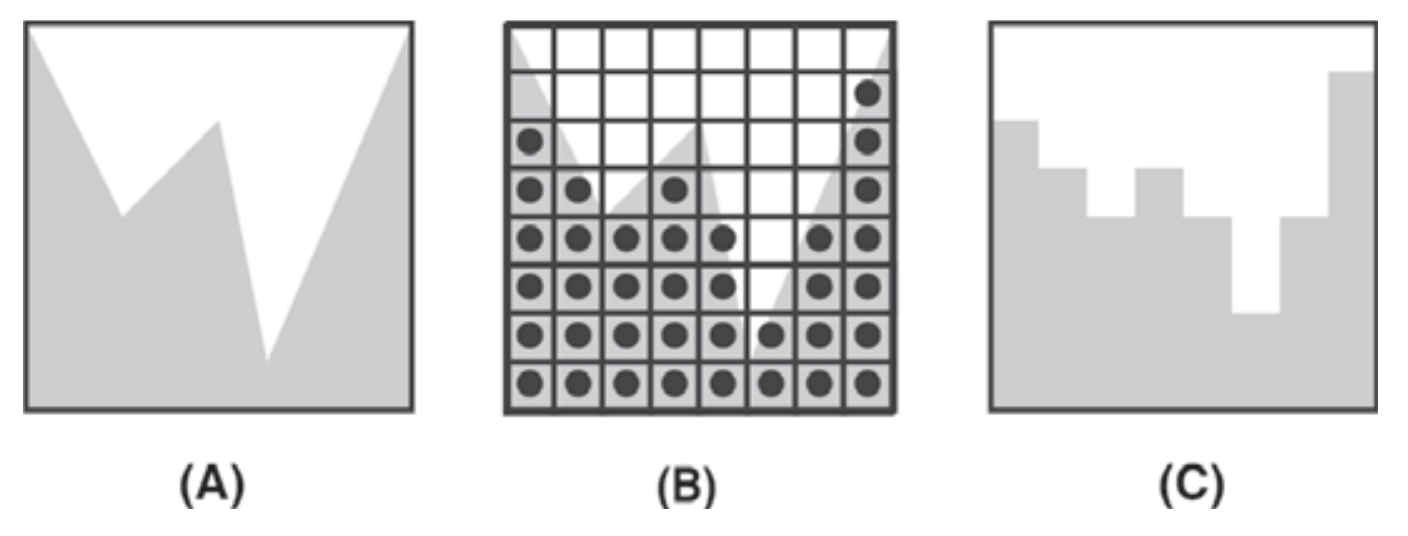
\includegraphics[width=\linewidth]{./figures/pointsampling.png}
    \end{figure}
\end{frame}

\section{Aliasing}

\begin{frame}[fragile]{Bordes geometría}
    \begin{figure}
        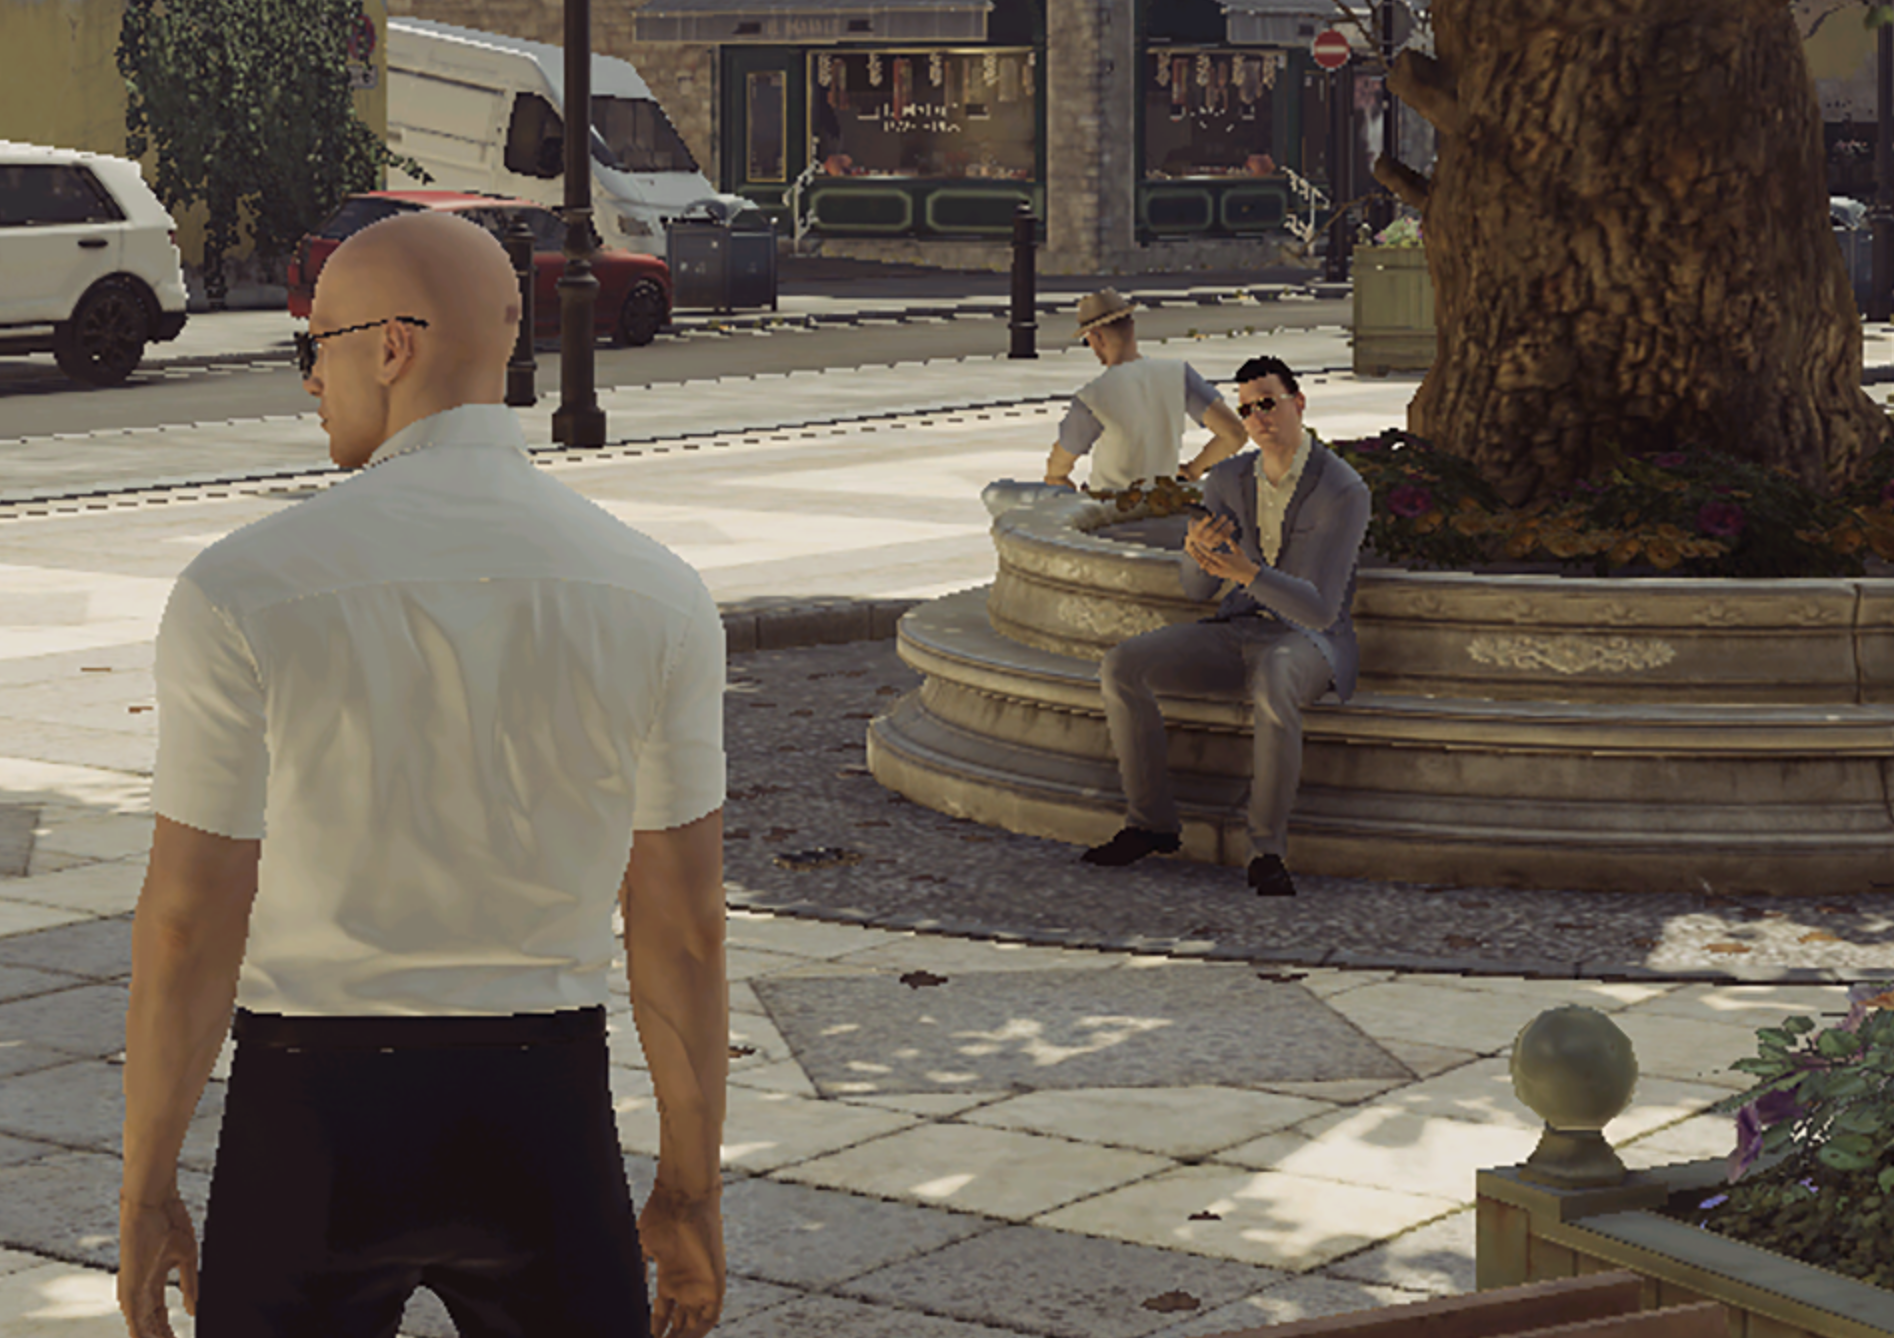
\includegraphics[width=\linewidth]{./figures/hitmanaliasing.png}
    \end{figure}
\end{frame}

\begin{frame}[fragile]{En textura}
    \begin{figure}
        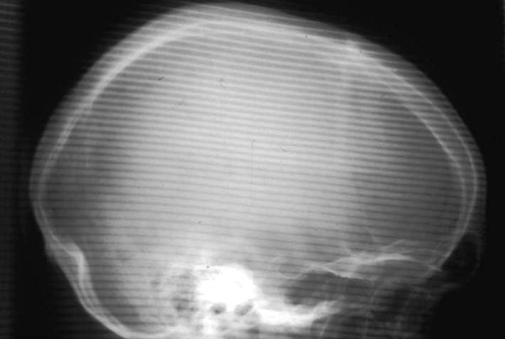
\includegraphics[width=.8\linewidth]{./figures/skull.jpg}
    \end{figure}
\end{frame}

\begin{frame}[fragile]{En textura}
    \centering
    \begin{figure}[!htbp]
        \centering
        \begin{subfigure}[b]{0.45\textwidth}
            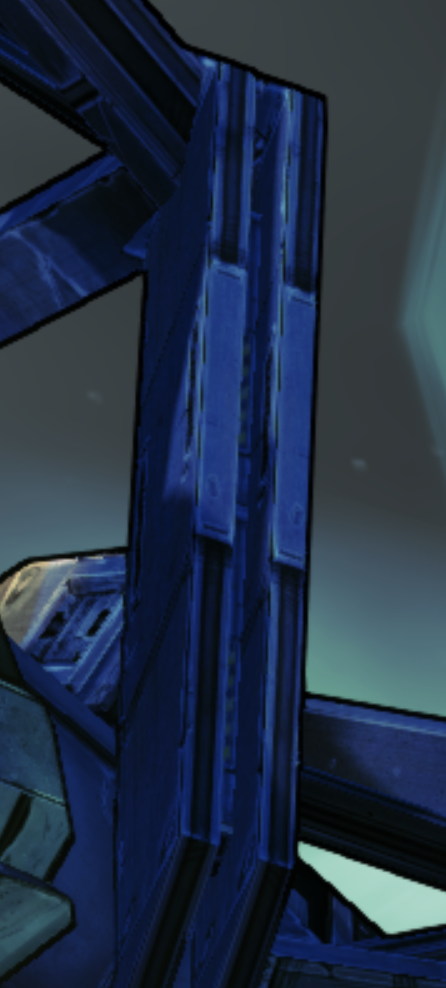
\includegraphics[width=\textwidth]{figures/ss2on.png}
        \end{subfigure}
        \centering
        \begin{subfigure}[b]{0.45\textwidth}
            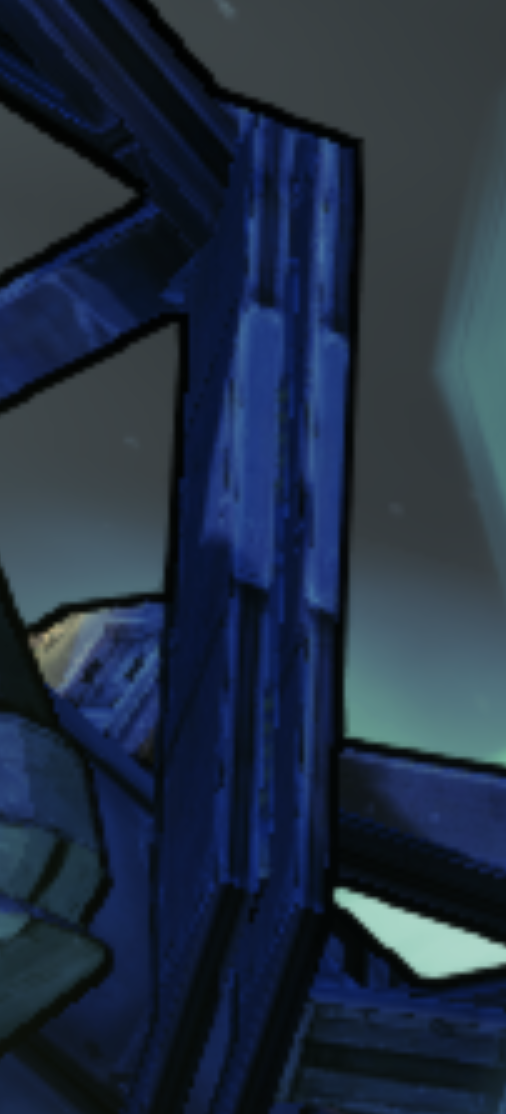
\includegraphics[width=\textwidth]{figures/ss2off.png}
        \end{subfigure}
    \end{figure}
\end{frame}

\begin{frame}[fragile]{Especular}
    \begin{figure}[!htbp]
        \centering
        \begin{subfigure}[b]{0.45\textwidth}
            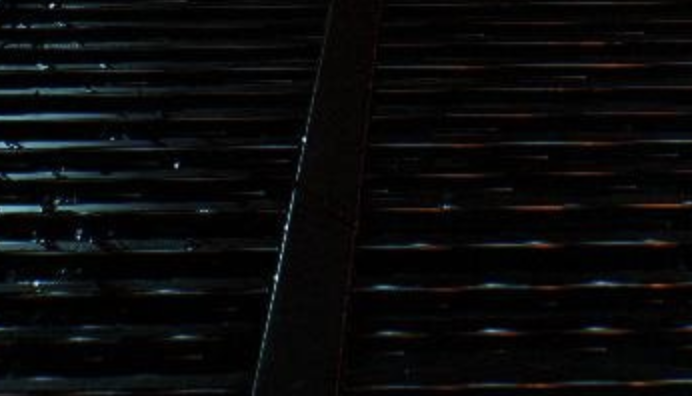
\includegraphics[width=\textwidth]{figures/specular-aliasing.png}
        \end{subfigure}
        \centering
        \begin{subfigure}[b]{0.45\textwidth}
            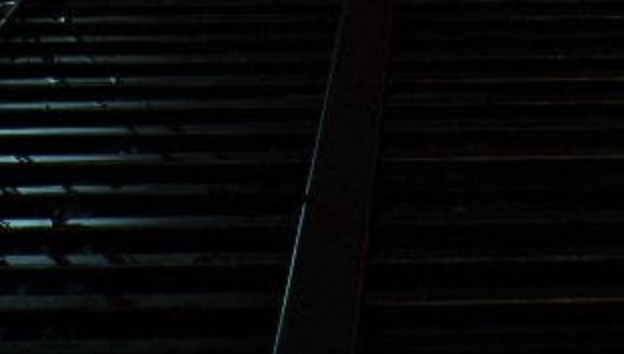
\includegraphics[width=\textwidth]{figures/specular-fixed.png}
        \end{subfigure}
    \end{figure}
\end{frame}

\section{Anti-aliasing tradicional}

\begin{frame}[fragile]{Filtros}
    \begin{figure}
        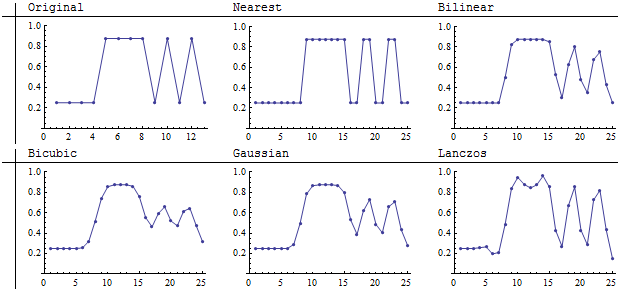
\includegraphics[width=\linewidth]{./figures/Lw6ei.png}
    \end{figure}
\end{frame}

\begin{frame}[fragile]{Filtros}
    \begin{figure}
        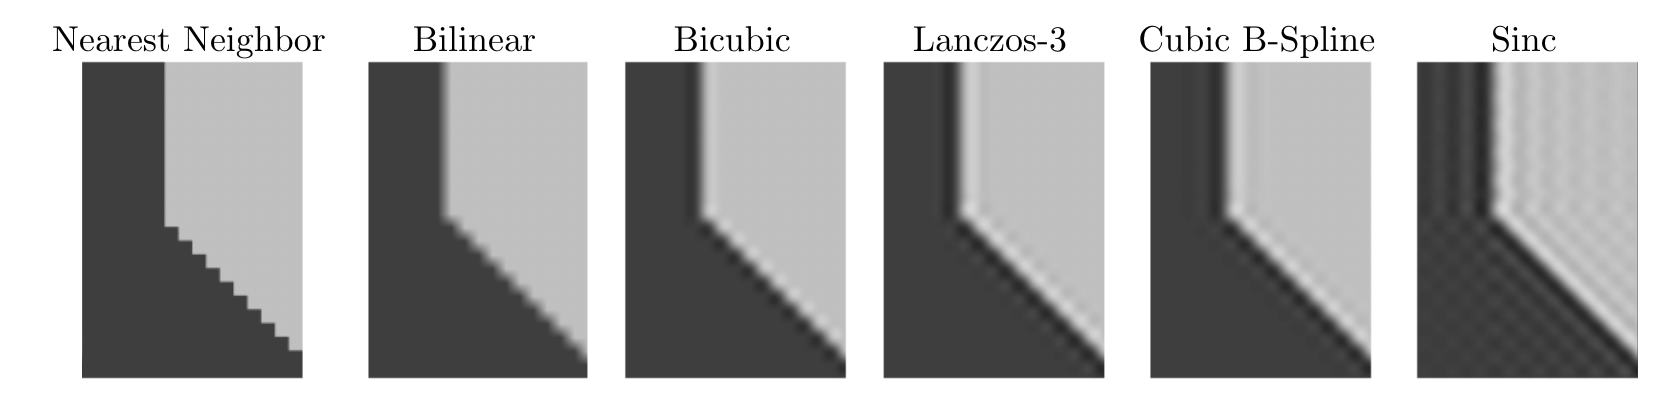
\includegraphics[width=\linewidth]{./figures/comparison-filter.png}
    \end{figure}
\end{frame}

\begin{frame}[fragile]{Supersampling}
    \begin{figure}
        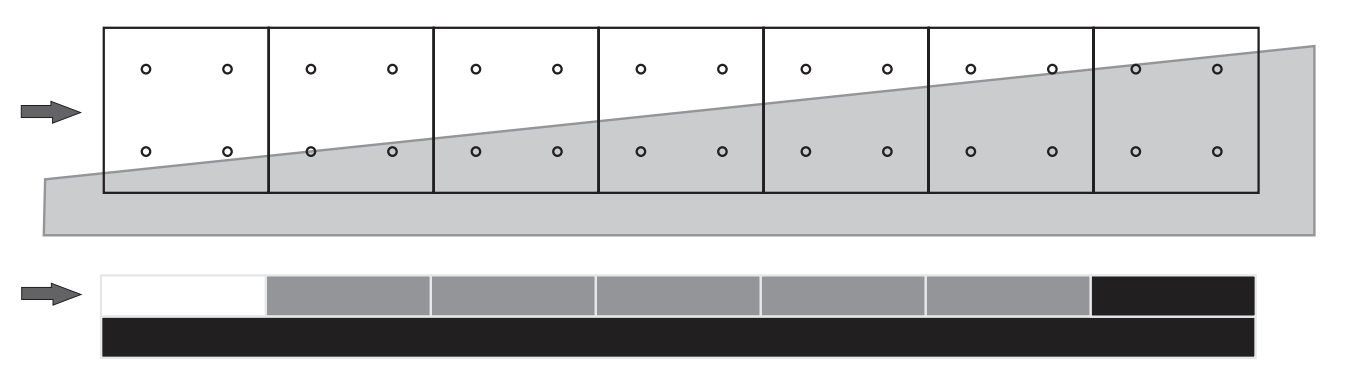
\includegraphics[width=\linewidth]{./figures/ogss.png}
    \end{figure}
    \begin{figure}
        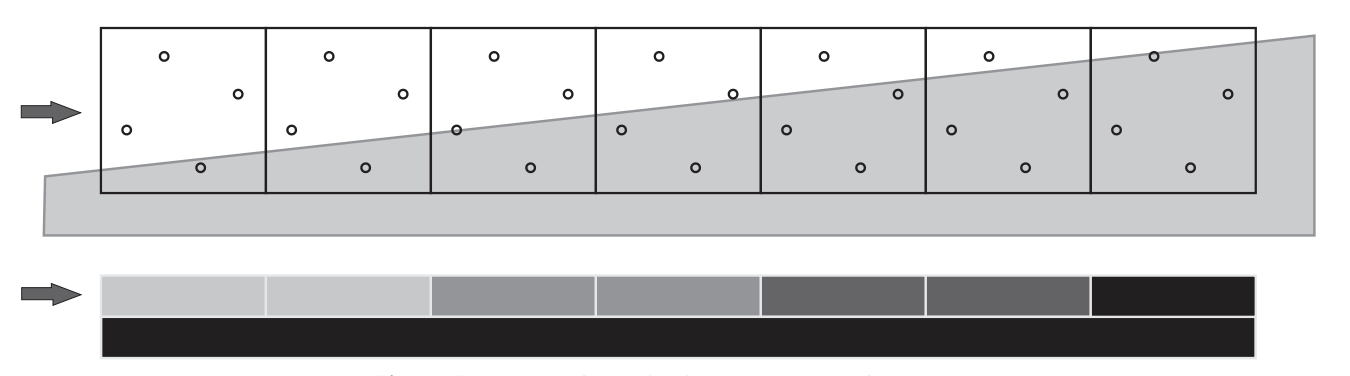
\includegraphics[width=\linewidth]{./figures/rgss.png}
    \end{figure}
\end{frame}

\begin{frame}[fragile]{Multisampling}
    No funciona con deferred shading

    \begin{figure}
        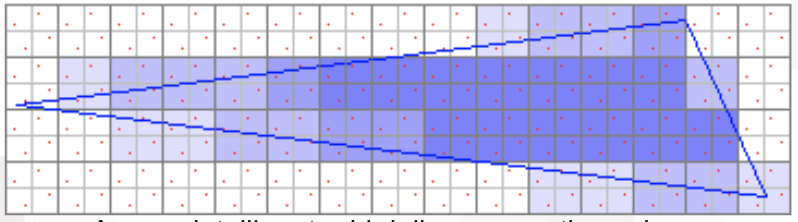
\includegraphics[width=\linewidth]{./figures/msaasample.png}
    \end{figure}
\end{frame}

\begin{frame}[fragile]{Post Processing AA}
    FXAA, MLAA, SMAA

    Inyección

    \begin{figure}[!htbp]
        \centering
        \begin{subfigure}[b]{0.45\textwidth}
            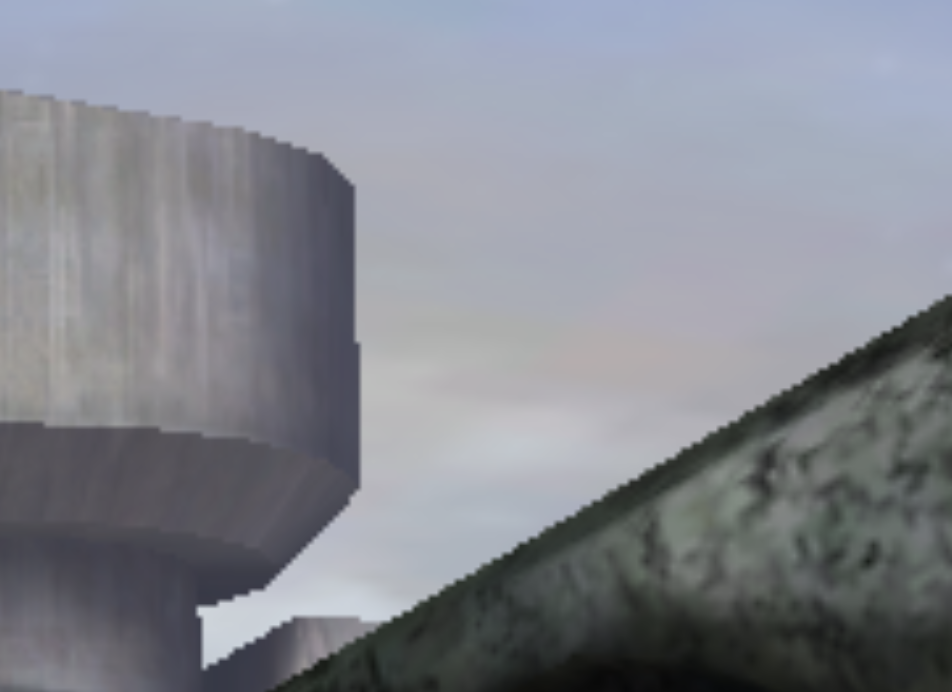
\includegraphics[width=\textwidth]{figures/smaaOFF.png}
        \end{subfigure}
        \centering
        \begin{subfigure}[b]{0.45\textwidth}
            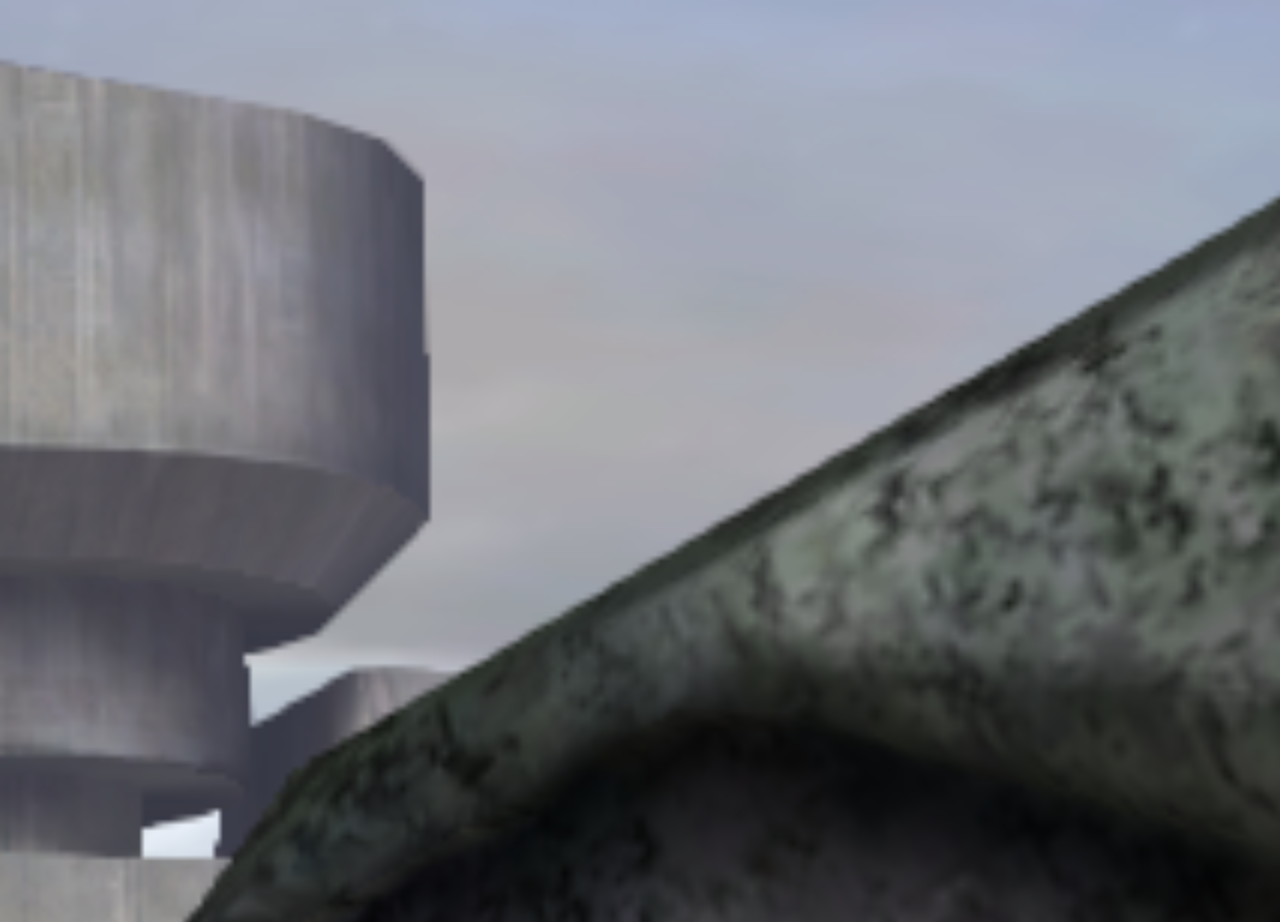
\includegraphics[width=\textwidth]{figures/smaaON.png}
        \end{subfigure}
    \end{figure}
\end{frame}


\section{Anti-aliasing temporal}

\begin{frame}[fragile]{History Buffer}
    Necesario guardar frame $n_{-1}$ para usar en shader

    \begin{figure}
        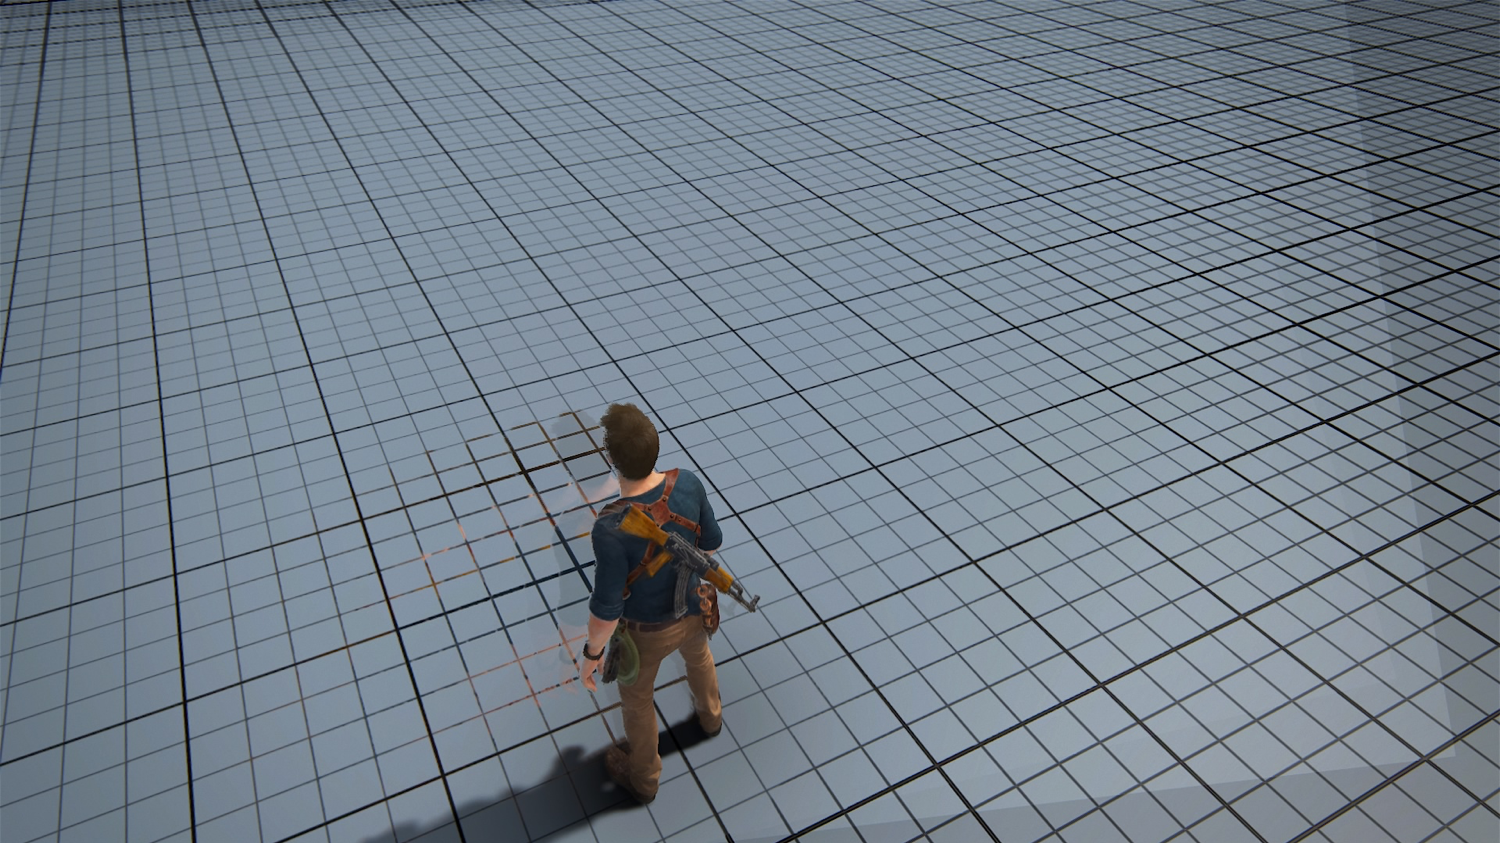
\includegraphics[width=\linewidth]{./figures/reprojection.png}
    \end{figure}
\end{frame}
\begin{frame}[fragile]{Jitter}
    Secuencias Halton

    Evita subsamples repetidos y clusters

    Aplicar jitter a $MVP$

    \begin{figure}
        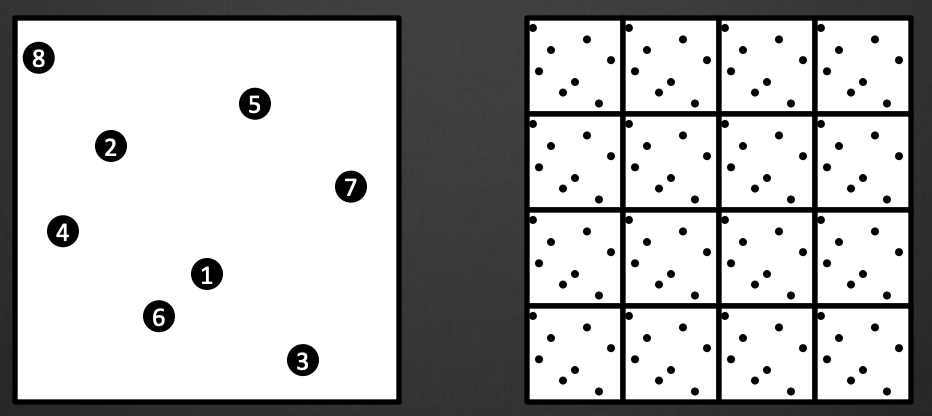
\includegraphics[width=\linewidth]{./figures/halton.png}
    \end{figure}
\end{frame}

\begin{frame}[fragile]{Velocity Buffer}
    \begin{figure}
        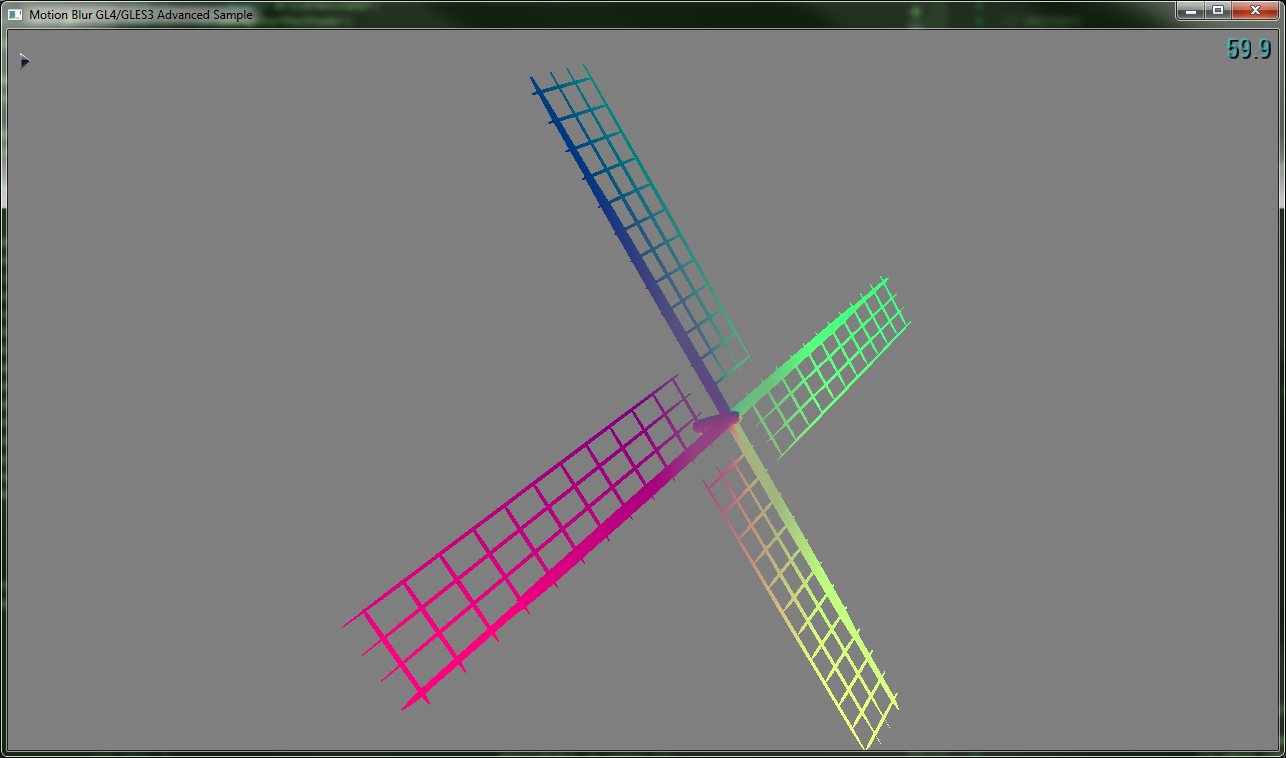
\includegraphics[width=\linewidth]{./figures/motionbluradvanced_velocity.png}
    \end{figure}
\end{frame}

\begin{frame}[fragile]{Clamping}
    Mirar pixels vecinos

    \begin{figure}
        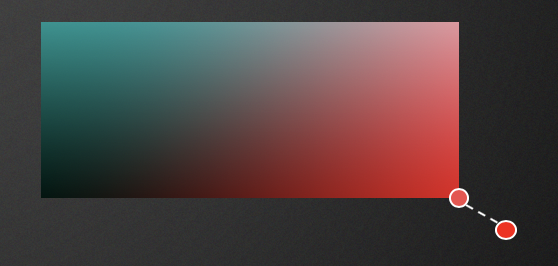
\includegraphics[width=\linewidth]{./figures/clamp.png}
    \end{figure}
\end{frame}

\begin{frame}[fragile]{Reprojection}
    Interpolación lineal (~5\%)
    \begin{figure}
        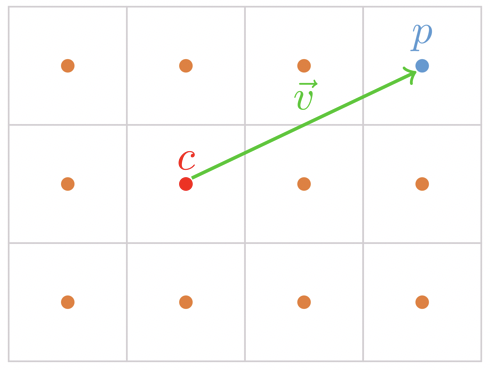
\includegraphics[width=.8\linewidth]{./figures/vec.png}
    \end{figure}
\end{frame}

\begin{frame}[fragile]{Sharpening}
    \[
        \begin{bmatrix}
            0 & -1 & 0 \\
            -1 & 5 & -1 \\
            0 & -1 & 0
        \end{bmatrix}
    \]
\end{frame}

\section{Resultados}

\begin{frame}[fragile]{Bordes geometría}
    \begin{figure}
        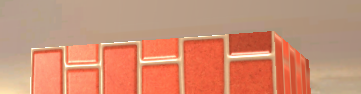
\includegraphics[width=.9\linewidth]{./figures/taaoff.png}
    \end{figure}
    \begin{figure}
        
\includegraphics[width=.9\linewidth]{./figures/taa8.png}
    \end{figure}
    \begin{figure}
        
\includegraphics[width=.9\linewidth]{./figures/taa16.png}
    \end{figure}
\end{frame}

\begin{frame}[fragile]{Especular}
    \begin{figure}
        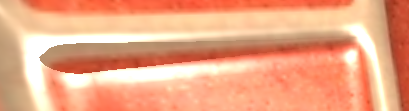
\includegraphics[width=\linewidth]{./figures/shadowtaaOFF.png}
    \end{figure}
    \begin{figure}
        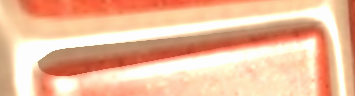
\includegraphics[width=\linewidth]{./figures/shadowtaaON.png}
    \end{figure}
\end{frame}

\begin{frame}[fragile]{Sharpening}
    \begin{figure}
        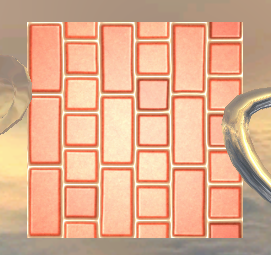
\includegraphics[width=\linewidth]{./figures/sharpOFFsmall.png}
    \end{figure}
\end{frame}

\begin{frame}[fragile]{Sharpening}
    \begin{figure}
        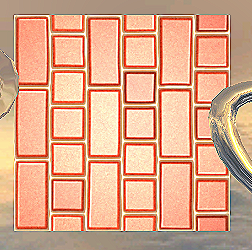
\includegraphics[width=\linewidth]{./figures/sharpONsmall.png}
    \end{figure}
\end{frame}

\section{Conclusiones y mejoras futuras}

\begin{frame}[fragile]{Conclusión}
    Rendimiento, calidad
    \begin{figure}
        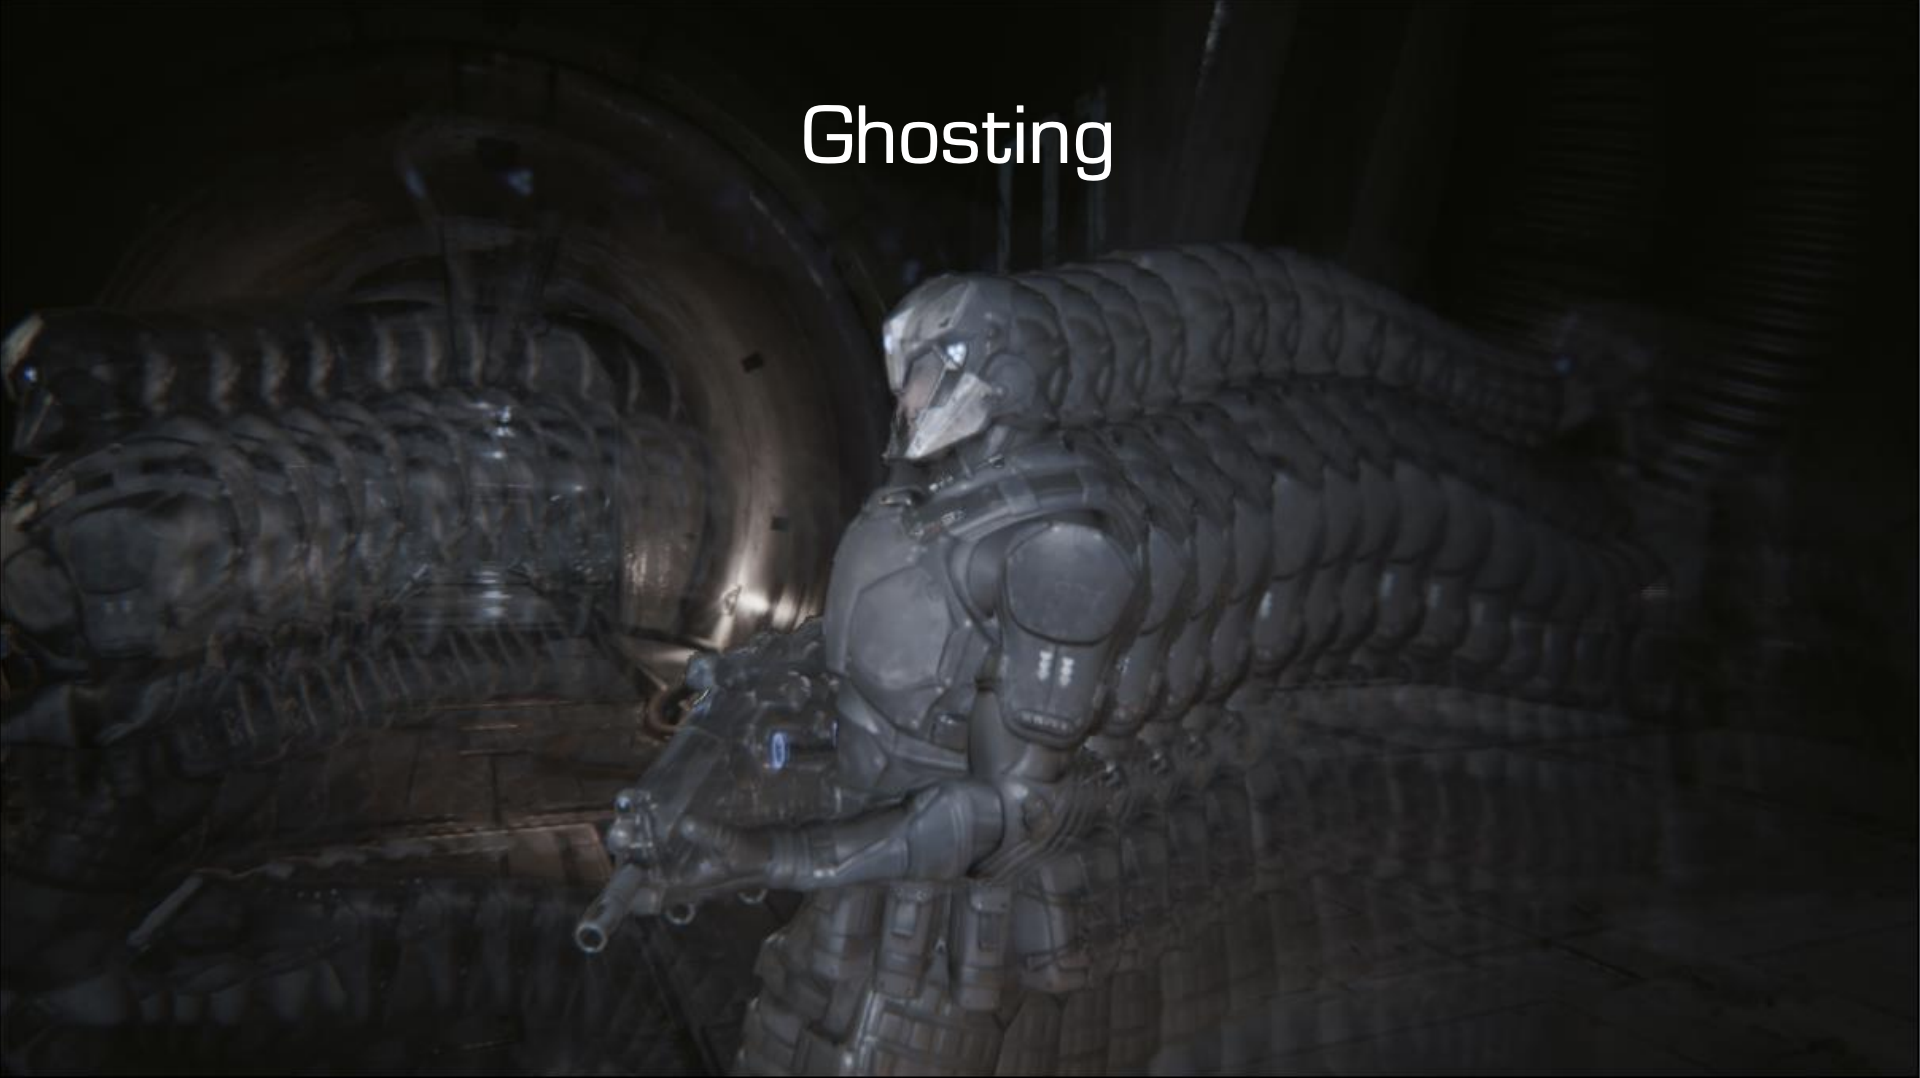
\includegraphics[width=.8\linewidth]{./figures/ghosting.png}
    \end{figure}
\end{frame}

\begin{frame}[fragile]{Mejoras}
    \begin{itemize}
        \item Blurring
        \item SSAO
        \item Transparencias
        \item Reflejos
    \end{itemize}
\end{frame}

\begin{frame}[fragile]{Blur}
    \begin{figure}
        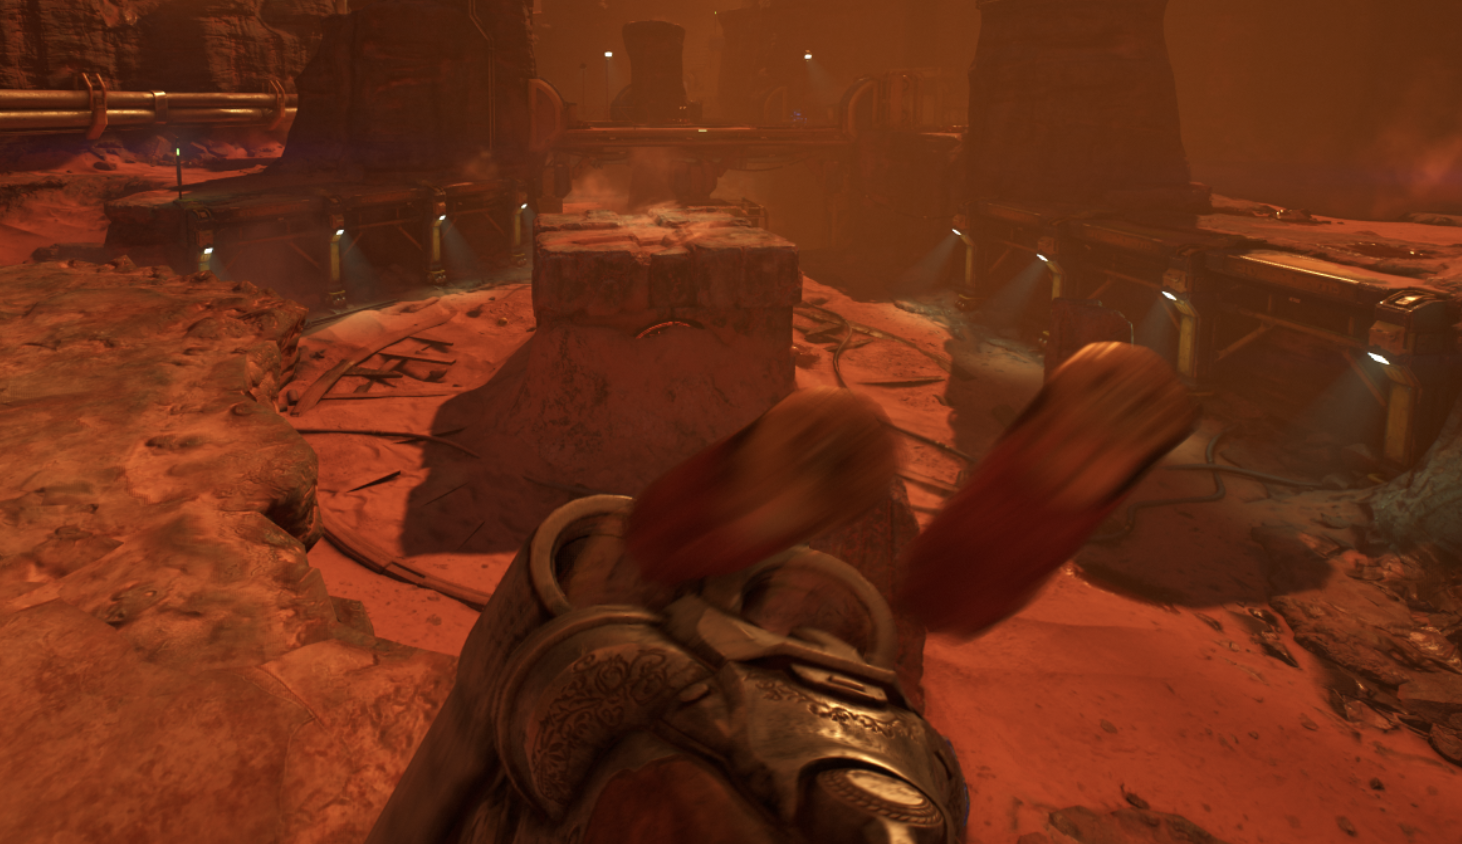
\includegraphics[width=\linewidth]{./figures/doomblur1.png}
    \end{figure}
\end{frame}


\begin{frame}[fragile]{Mejoras}
    \begin{figure}
        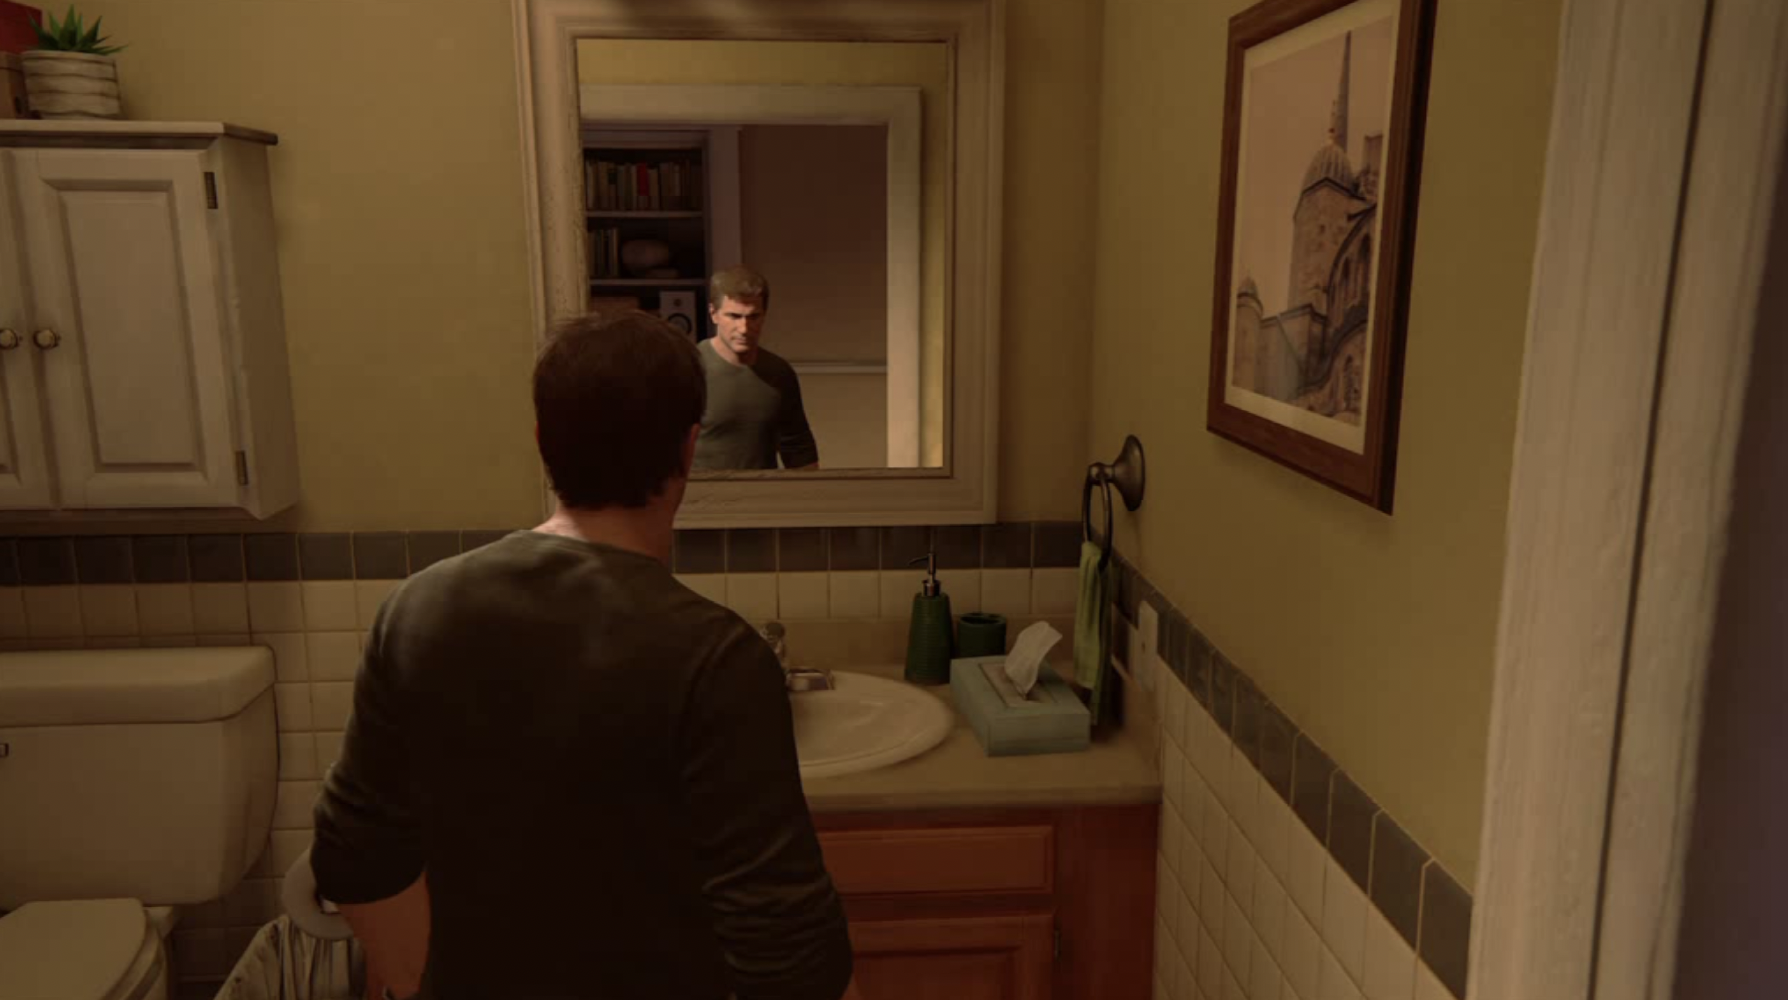
\includegraphics[width=\linewidth]{./figures/reflection.png}
    \end{figure}
\end{frame}

\begin{frame}
    \titlepage
\end{frame}
\end{document}
